\subsubsection*{Methodology of the ASIC subproject.}

The front-end electronics (FEE) Data acquisition (DAQ) and slow controls (SC) 
for P0 and P4 will also use the solutions which have been jointly developed between NEXT, CERN and other institutions (who joined later the project) for the CERN RD-51 collaboration. We describe them briefly here. 

\paragraph{A DAQ solution for P0/P4:}
%
We propose to use the NEXT/RD-51 DAQ system, named SRS \footnote{S.Martoiu et al., JINST (8) 2013, DOI: 10.1088/1748-0221/8/03/C03015,J .Toledo et al, JINST (6) 2011, DOI: 10.1088/1748-0221/6/11/C11028.}, which has been licensed to an European company, EicSys, and ported to the industry standard ATCA.
%
The main SRS-ATCA components are: (1) An ATCA chassis, which includes power, cooling fans and a shelf manager unit for remote monitoring and control via Ethernet; (2) ATCA blades, which are carriers with mezzanine connectors, memory, processing units (FPGAs) and I/O connectivity; and (3) mezzanine cards to adapt to a wide range of front ends. Operation with the NEXT-DEMO and NEXT-NEW detectors has shown the stable and reliable operation of SRS-ATCA. 

The ADC mezzanines can achieve 60 MHz sampling rate. P0 will have one LXSC6 ($64 \times 6 = 384$~channels) and P4 will have 4 LXSC2 ($64 \times 8 = 512$~channels reusing also those previously deployed in P0).Each mezzanine handles 24 channels. Thus, 22 mezzanines will provide 528 channels.  

Each ATCA blade carries two mezzanines. So, 12 ATCA blades are required, fitting in a 12-slot  ATCA chassis. Ot these, 11 blades are used for digitisers (512 channels) and 1 blade for TDCs. The ATCA blades send data to a DAQ PC farm. Experience with the NEXT experiment, indicate that for good performance, 14 DAQ PCs would be needed (10 for Local Data Concentrators, 3 for Global Data Concentrators and one as a Storage PC). 

%
\paragraph{A solution to achieve high time resolution in P0/P4:}
%
One of the most promising applications of PETALO is to function as TOF-PET. This requires excellent time resolution. Fortunately, a ready solution also exist. In the near future, EicSys will be upgrading their ATCA blades to include WhiteRabbit\footnote{[3] http://www.ohwr.org/projects/white-rabbit} nodes in its I/O section. WhiteRabbit is a CERN development used to synchronise thousands of elements in a distributed DAQ and control system across kilometre distances with sub-nanosecond resolution. In small setups like a PET, synchronisation within 200 picoseconds can be achieved with a careful calibration process. WhiteRabbit is an extension to GbE over fibre optics and uses SFP transceiver modules.
%
%%A similar approach was developed by a former member of out research group at UPV, showing better performance in some aspects. White Rabbit is open hardware and so the firmware is freely available. Thus, we must invest effort (three months sound reasonable) in reducing as much as possible skew and jitter in the White Rabbit network, as this will be the main limitation to the time resolution in the PET. This implies potential enhancements in the synchronization protocols, in electronic componentes and in network architecture.
%
%%A Spanish company based in Granada, named Seven Solutions [ref4], develops and provides solutions based on WhiteRabbit. Apart from the WhiteRabbit nodes in the ATCA blades, which will be equipped by EicSys, we need the following elements from Seven Solutions to enhance the timing resolution for PETALO-2: (1) two 18-ports WhiteRabbit switches, which are a special kind of GbE switches to build the WhiteRabbit network and (2) a White Rabbit plug-in module (named WR-LEN) to provide reliable timestamps for the TDC module which will be explained in the section devoted to PETALO-2 front-end.
%

Consequently the 512 ADC channels needed by P4 can operate across the ATCA chassis with a controlled clock phase and with a reference timestamp. An additional benefit is the availability of 512 TDC channels which will accurately provide TOF and DOI timestamped information, which in turn can be used to trigger the acquisition. Front-end boards for slow and fast paths for 64 channels, thus matching a 64-SiPM dice board, will be designed, as discussed below.
%
%
\paragraph{A front end for P4}
%
The SiPMs which we plan to use in the LXSC (SENSL 6mm C/J series)
operating inside the cryostat will have a gain of 10$^7$. According to our initial Monte Carlo simulations, the required dynamic range varies from 20 to 2000 photoelectrons.  This can result in a large signal current of several milliamps. With more than 20.000  pixel cells, the SiPM output will be extremely linear. Moreover, dark count noise will be negligible at cryostat temperatures. The only effect to deal with will be optical crosstalk between neighbouring cells. %These SiPMs have and additional fast output that could be used in addition to the conventional one (anode or cathode) for the fast timing channel.

The SiPM signal will have an extremely fast rising edge with a fast decay time constant of 2 ns followed by a longer (though still fast) tail with a decay time constant of 45 ns. As a result, excellent timing resolution can be achieved with SiPMs to produce TOF and DIO information. We plan to amplify (current to voltage conversion with a fast operational amplifier) the output for all SiPMs and connect the amplified signals to TDC chips, having as reference the low-jitter system clock produced by the WhiteRabbit interface. The 8-channel THS788 TDC from Texas Instruments has 13 ps resolution, with 8 ps accuracy (sigma). This would produce very accurate timestamps for the scintillation light. 
%Take into account that 30 ps represents in liquid Xe  approx. 6,6 mm. 
Eight such TDCs would allow to timestamp 64 channels (one DB).

At the same time, good spatial and energy resolution are required. All channels will be converted to voltage with an operational amplifier, stretched to adapt to the sampling rate and adapted to the dynamic range of the ATCA mezzanine digitising card.

The slow, analog outputs will be connected via HDMI cables to the ATCA digitiser boards. The TDC outputs will be formatted in an FPGA and sent to an ATCA blade, adapted via an LVDS digital interface developed for the NEXT detector.
%
%\paragraph{Scaling up to PETALO-10}
%
%P10 will instrument 10 LXSC2 for a total of 20 DBs. Re-using the electronics of P2 (8 DBs), we need the FEE and DAQ for 12 additional DBs. 

\paragraph{Development of FEE, DAQ and Slow control for P0/P4:}

Since PETALO will use COTS (commercial off the shelf), extensively tested (by NEXT/RD-51) solutions for FEE and DAQ the components can be ordered without delay as soon as the project starts. Assuming the nominal starting data in January-16, the full system can be ready in 3 months, allowing 3 more months for testing, firmware, and validation before the start of operations foreseen for P0. In brief:  
\begin{enumerate}
\item Acquisition of ATCA DAQ and FEE system (including chasis, blades, digitisers and TDCs) corresponding to 8 DBs  (Q1-16).
\item Testing of ATCA system (Q2-16).
\item Development Slow Controls (Q1/Q2-16)
\end{enumerate}

%\paragraph{Development of FEE, DAQ and Slow control for P10: Methodology}
%
%Operation of P2 during Q3/Q4-16 will certify the whole system. Since P10 will be based in the same solutions tested in P2, the scalability is straight forward. We plan to reuse the ATCA system of P2 to reduce costs (which corresponds to 8 DBs). Since P10 deploys LXSC2 cells, one needs to readout 20 DBs, and therefore we need to order 12 additional DBs for P10. This will be done in the first quarter of 2017, so that the ATCA system will be ready in Q2-17 to start operations with P10. Therefore:  
%
%\begin{enumerate}
%\item Acquisition of ATCA DAQ and FEE system for 12 additional DBs  (Q1-17).
%\item Testing of full system (Q2-17).
%\item Development Slow Controls for P10 (Q1/Q2-17)
%\end{enumerate}
%
%The slow control will also be based in the same solution adopted for NEXT (RIO modules).
%
\paragraph{Development of an ASIC optimised for PETALO (APE):}

While the solutions for the FEE and DAQ proposed by P0/P4 will allow fast and reliable operation for the proof-of-concept, a more compact and economical solution is needed for a clinical PET, specially, if, as it is the case of PETALO, the low cost of the detection unit (compared with SSDs) makes it feasible, a priory to build a large ``full body'' apparatus. On the other hand, since the detector offers such an excellent performance in terms of energy and time resolution, it is mandatory that the integrated front-end does not degrade overall system performance.

\paragraph{APE. Costs and Alternatives:}

Since the key point of the integrated solution lies in the ADC element a state-of-the-art survey has been done in order to evaluate the trade-offs of the design \footnote{J.M. de la Rosa: “Sigma-Delta Modulators: Tutorial Overview, Design Guide and State-of-the-Art Survey,” IEEE Trans. on Circuits and Systems - I: Regular Papers, vol. 58, pp. 1-21, January 2011.}. For COTS ADCs the corner point in terms of ENOB (effective number of bits) vs. Samples per second lies around 14 bits / 200 MSamples. This means that an ASIC of the specifications required by PETALO, where there are a huge number of channels to acquire and many sensitive elements lie close to the ADC, will never reach this optimum. Bearing in mind that the most advanced technology node available for the research team is 180 nm, a realistic approach to this situation would recommend a safe operation zone in the order of 10-12 bits / 10-20 MSamples.
 
To minimise dead time a charge integrator will be introduced in the front-end, so that the energy of the incoming pulse is obtained. Thus only one data is converted for every channel during a certain event. If the integrator is carefully designed the full pulse energy can be measured with an excellent dynamic range. If a high precision ADC is used an excellent resolution might be achieved. The system dead time can be reduced below 1 microsecond.

The design process of the integrated front-end is divided in two stages. The first one will produce a prototype able to implement an ADC conversion and produce a trigger signal which will make use of the WhiteRabbit infrastructure to implement time coincidence. Basically it will be an upgrade of the existing DAQ system with the ADC conversion moved up close to the detector output. The second one will produce a final front-end solution to implement a scalable fully functional read-out system for a high performance PET system. Thus it must implement a synchronisation scheme to be able to produce coherent time-stamps for the detected events throughout the system.  
%\begin{itemize}
%    \item Analog Memory Sampling
%    \begin{itemize}
%      \item Effective Sampling Time (pulse length 320 ns): 10 ns
%      \item Type of ADC: Nyquist (SAR, Pipeline, tbd.) 10-12 ENOB
%      \item Number of ADCs: 4 (8 channels per ADC)
%      \item Deadtime (20 MSamples): 12.8 $\mu$s
%      \item AREA(mm$^{2}$): Preamplifier(1.92) / Analog Memory(0.64) / ADC(4) / Transceivers + Pads + Routing etc. (2) = TOTAL (8.56)
%      \item COST for 40 devices (needed for PETALO 10): Without TDC (22620 Euros ) / With TDC (26600 Euros)
%    \end{itemize}
% 
% 
%    \item Charge Integration Front-end
%    \begin{itemize}
%      \item Effective Sampling Time (pulse length 320 ns): N.A. (Pulse Integration)
%      \item Type of ADC: Oversamplig (Sigma-Delta) 12 ENOB
%      \item Number of ADCs: 4 (8 channels per ADC)
%      \item Deadtime (8 MSamples): 1 $\mu$s
%      \item AREA(mm$^{2}$): Preamplifier(1.92) / Integrator(2,56) / ADC(4) / Transceivers + Pads + Routing etc. (2) = TOTAL (10.56)
%      \item COST for 40 devices (needed for PETALO 10): Without TDC (24450 Euros ) / With TDC (284400 Euros)
%    \end{itemize}
%\end{itemize}

\paragraph{Integrating the first version of APE in P4:}
The first version of APE integrates the SiPM output current for as long as it stays over a programmable threshold. This time-over-threshold integration produces an output proportional to the pulse energy. 
%Once digitized, this value is far more compact, in terms of data throughput, than a sequence of digitized samples. But the real advantage of this approach is a large reduction in the ASIC dead time.
Thus, the ASIC replaces the front-end path (front-end board and ATCA ADC mezzanine) in the discrete implementation used for P4. In order to integrate the ASIC in the ATCA DAQ system, the ATCA chassis and blades are re-used and the ADC mezzanines, which are not required anymore, are replaced with digital interface ATCA mezzanines developed in the framework of the NEXT project. As a result, the only new development will be a carrier board for the ASICs with some glue logic to interface the ATCA digital mezzanines.
 
 \paragraph{Development of APE: Methodology}
 
 \begin{figure}[!htb]
	\centering
	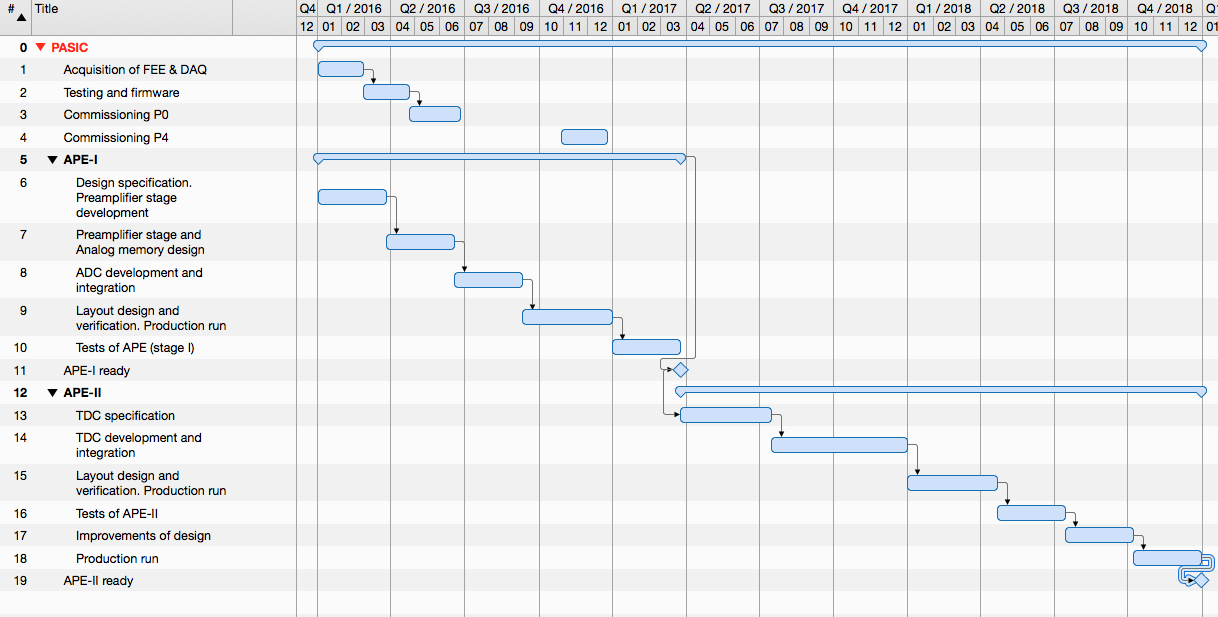
\includegraphics[scale=0.4]{img/ASICWF.png}
	\caption{\label{fig.ASICWF} Work flow of activities for ASIC.  }
\end{figure}

 
The design of APE will start early in the project, and will proceed in parallel with the development of P2 and P10. This will permit a first production run in 2016, and the possibility of testing the first stage in P2 during the first quarter of 2017. If the tests are successful P10 could then be equipped with the ASIC units rather than with discrete ADC cards. Specifically the lists of tasks and the development period is:

\begin{enumerate}
\item Design specification. Preamplifier stage development (Q1-16).
\item Analog memory design (Q2-16).
\item ADC development and integration. (Q3-16)
\item Layout design and verification. Production run (Q4-16)
\item Tests of APE in P4 (Q1/17)
\end{enumerate}
 
 The design of the full ASIC will then proceed during Q2/Q4-17, with the aim of a production run in Q1-18 and testing in P2 in Q2-18. If needed, a second run will occur in Q3-18, followed by testing in Q4-18. Figure \ref{fig.ASICWF} shows a flow diagram. 
